\begin{figure}[htbp]\centering
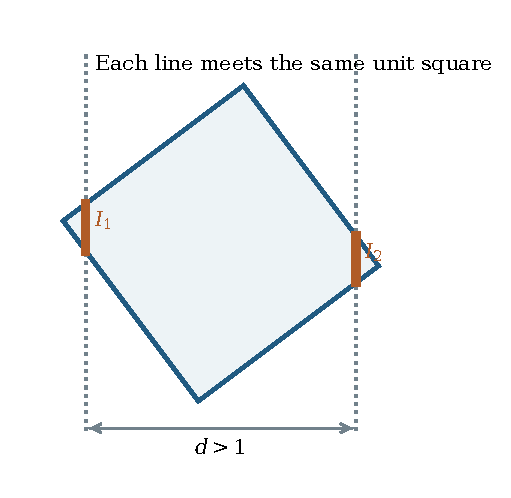
\includegraphics[width=.72\textwidth]{figures/03_parallel_chords.pdf}
\caption{Two nonempty parallel chords of the same unit square.
A tangent point is nonempty even though its chord length is zero.}
\label{fig:parallel}\end{figure}

\begin{lemma}[Endpoints of a singly filled gap]\label{lem:closed-gap}
If a nonempty open segment $(A,B)$ lies in one fixed closed tile $K$,
then both $A$ and $B$ belong to $K$.
\end{lemma}
\begin{proof}
Take sequences in the open segment converging to its two endpoints and use
closedness of $K$. If only $K_1\cup K_2$ is known to contain the gap,
the argument does not put both endpoints in either specified tile.
\end{proof}

\begin{figure}[htbp]\centering
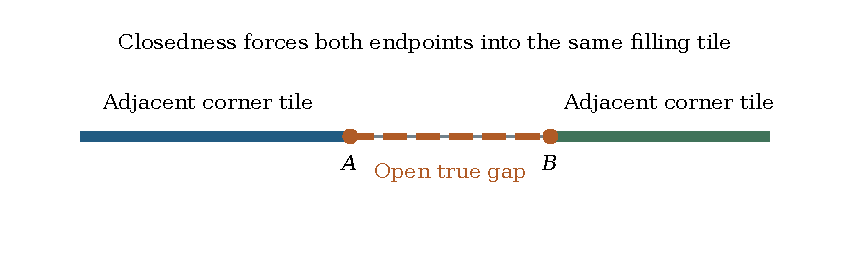
\includegraphics[width=.97\textwidth]{figures/05_gap_endpoints.pdf}
\caption{The same filling tile must first be identified for the entire open
gap. Only then does closedness give both endpoints.}
\label{fig:gap}\end{figure}
